% Paper 2 manuscript (Prompt 15). IEEE conference format, for Overleaf.
% Evidence rules: every number comes from a file listed in evidence_checklist.md.
% [TO FILL: ...] = result not yet produced (main runs after the freeze).
% [TO VERIFY: ...] = fact not yet checked.
\documentclass[conference]{IEEEtran}
\usepackage[utf8]{inputenc}
\usepackage[T1]{fontenc}
\usepackage{amsmath,amssymb}
\usepackage{graphicx}
\usepackage{booktabs}
\usepackage{xcolor}
\usepackage{url}
\usepackage{tikz}
\usetikzlibrary{positioning,arrows.meta}
\usepackage[hidelinks]{hyperref}

\newcommand{\tofill}[1]{\textcolor{red}{[TO FILL: #1]}}
\newcommand{\toverify}[1]{\textcolor{orange}{[TO VERIFY: #1]}}
\newcommand{\Sp}{S_{\mathrm{prompt}}}

\begin{document}

\title{Rewording or Re-Sampling? Separating Prompt and Sampling
Instability in LLM Conclusions on Biomedical Evidence}

\author{\IEEEauthorblockN{Patel Dhruv Rajendrakumar}
\IEEEauthorblockA{M.Tech in CLIS, Roll No.\ MCL2026002}\\
}

\maketitle

% The abstract was written last, to match the evidence in the paper.
\begin{abstract}
When a large language model (LLM) is asked to draw a conclusion from
research evidence, its answer can change when the prompt is reworded and
when the same prompt is simply run again. Earlier studies measured either
cross-prompt consistency or sampling variation, but not both for
evidence-based conclusions with an expert reference. We describe a
pre-registered controlled comparison that splits the label disagreement of
Qwen2.5-7B-Instruct on PubMedQA into a between-prompt and a within-prompt
part, compares three ways of obtaining the model's conclusion, and tests
whether the measured instability depends on the scoring method. Before any
test item is used, we validate the baseline on the 500 development items:
the canonical prompt reaches an accuracy of 0.588 (95\% CI 0.544--0.628)
and macro-F1 0.553, which is not significantly above always answering
``yes'' (0.552; exact McNemar $p = 0.27$). Most of its errors (170 of 206)
are hedges, where an expert ``yes'' or ``no'' is answered ``maybe''. On 100
development items, asking for the conclusion before the label raised
accuracy from 0.56 to 0.72 (Holm-adjusted $p = 0.003$), while 8-bit instead
of 4-bit weights changed nothing detectable. The output format, not the
quantisation, therefore drives the baseline's hedging; because the variant
was designed on the same items, the size of the gain is likely
overstated.
\end{abstract}

\begin{IEEEkeywords}
prompt sensitivity, sampling variability, self-consistency, biomedical
question answering, evaluation reliability, PubMedQA
\end{IEEEkeywords}

% =====================================================================
\section{Introduction}
LLMs are increasingly used to read research evidence and state what it
implies. A conclusion produced this way is only useful if it does not
depend on incidental choices. Two such choices are well documented. First,
small changes to the wording or format of a prompt can change the
answer~\cite{lu2022fantastically,zhao2021calibrate,chatterjee2024posix,zhuo2024prosa,errica2025what}.
Second, running the same prompt again with sampling can give a different
answer~\cite{cui2026same}. Evaluations that use a single prompt and a
single run cannot tell these two sources apart, and multi-prompt
evaluation has been proposed for exactly this reason~\cite{mizrahi2024state}.

The closest prior work measured each source separately.
Hariprasad~\cite{hariprasad2026prompt} reported cross-prompt answer
consistency of small open models on medical question answering, including
PubMedQA, at temperature 0 with one run per prompt; with one run, sampling
variation cannot be separated from prompt variation. Haase et
al.~\cite{haase2026within} partitioned prompt and within-model sampling
variance, but for creative tasks without a ground truth. As far as the
pages of these two papers show, neither splits prompt and sampling
variation for evidence-based conclusions with an expert reference. This
combination is the difference this study investigates. It is a
controlled measurement study, not a new method, and the novelty claim
stays provisional until our literature search is complete.

We ask three research questions on PubMedQA~\cite{jin2019pubmedqa}, where
each item is a research question with a biomedical abstract whose
conclusion has been removed, and the expert label is yes, no or maybe:
\begin{itemize}
\item \textbf{RQ1 (primary).} What share of the label disagreement comes
from rewording the prompt rather than from re-sampling it?
\item \textbf{RQ2.} Do a single greedy prompt, self-consistency on that
prompt~\cite{wang2023selfconsistency} and a majority over several
prompts~\cite{mizrahi2024state} report different conclusions?
\item \textbf{RQ3.} Does the measured instability depend on whether the
label field is parsed, the free-text conclusion is read by an LLM judge,
or it is read by a human~\cite{hua2025flaw}?
\end{itemize}

\noindent\textbf{What is ours and what is not.} The decomposition uses the
Gini impurity, and the estimators and scoring methods come from published
work~\cite{wang2023selfconsistency,mizrahi2024state,hua2025flaw}. Our
contributions are: (i) a pre-registered protocol that applies the
decomposition to evidence-based conclusions with an expert reference; (ii)
a validated, reproducible baseline, with the finding that its output
format drives most of its errors (Section~\ref{sec:results}); and (iii)
the RQ1--RQ3 measurements . Statements about why the
model behaves as it does are marked as conjectures.

% =====================================================================
\section{Related Work}
\textbf{Prompt sensitivity.} Few-shot results depend on example
order~\cite{lu2022fantastically} and on label bias that can be
calibrated~\cite{zhao2021calibrate}. Sensitivity has been summarised in
indices such as POSIX~\cite{chatterjee2024posix} and
ProSA~\cite{zhuo2024prosa}, and studied for prompt-engineering
choices~\cite{errica2025what}, for underspecified classification
prompts~\cite{pecher2026revisiting}, and in a more general
analysis~\cite{liu2026understanding}. Mizrahi et
al.~\cite{mizrahi2024state} showed that single-prompt rankings are
brittle and proposed multi-prompt metrics (MaxP, AvgP, CPS), which we
report for RQ2.

\textbf{Sampling and reproducibility.} Identical settings can still give
different outputs: Cui and Alexander~\cite{cui2026same} found this for
LLM-based data analysis, and Haase et al.~\cite{haase2026within} measured
within-model against between-prompt variance for creative tasks.
Self-consistency~\cite{wang2023selfconsistency} turns sampling variation
into an estimator by majority vote over samples; it was shown on
reasoning tasks with chain-of-thought~\cite{wei2022chain}, not on 3-way
evidence labels.

\textbf{Scoring artifacts.} Hua et al.~\cite{hua2025flaw} argued that part
of the measured prompt sensitivity is an artifact of rigid answer
extraction, and that an LLM judge reduces it. RQ3 tests whether this holds
when the model returns a structured label field.

\textbf{Medical question answering.} Hariprasad~\cite{hariprasad2026prompt}
measured cross-prompt consistency on PubMedQA and other medical sets.
Thapa et al.~\cite{thapa2025disentangling} report 73.9\% for
Qwen2.5-7B-Instruct on PubMedQA when the model selects an answer directly
(1{,}000 questions, temperature 0.2, full precision); their prompt and
whether the abstracts were given are not stated, so we use the number only
as a reference point.

% =====================================================================
\section{Methodology}
\label{sec:method}
\subsection{Task, data and splits}
We use the 1{,}000 expert-labelled PQA-L items of
PubMedQA~\cite{jin2019pubmedqa} (repository commit \texttt{1cbae8e9}) in
the reasoning-required setting: the model sees the question and the
abstract without its conclusion, and the gold label is
\texttt{final\_decision}. The official split script, run unchanged, gives
500 test and 500 development items; both have 276 yes, 169 no and 55 maybe
labels. All prompt writing, piloting and baseline validation use only
development items. The test pool is locked by a code guard until the
protocol is frozen.

\subsection{Prompts}
The canonical prompt P0 asks for one JSON object with the fields
\texttt{decision} (yes/no/maybe), \texttt{conclusion} (one sentence) and
\texttt{certainty} (high/moderate/low), in that order, under a fixed system
message (full text in \texttt{configs/prompts.yaml}). Five paraphrases P1--P5 change only the instruction wording; they
keep the evidence, the question, the output schema and the field order,
and must not change the audience, the evidence standard or the decision
criterion. Each paraphrase is checked by the author and one peer. A question-only control removes the
abstract.

\subsection{Decomposing disagreement (RQ1)}
For item $i$, prompt $j \in \{1,\dots,m\}$ ($m = 6$) produces $k = 5$
sampled labels. Let $p_{ij}(c)$ be the share of label
$c \in \{\text{yes},\text{no},\text{maybe},\text{invalid}\}$ among them and
$\bar p_i(c) = \frac{1}{m}\sum_j p_{ij}(c)$. The total disagreement is the
Gini impurity of all $mk$ labels,
\begin{equation}
G_i = 1 - \sum_c \bar p_i(c)^2 ,
\end{equation}
and it splits exactly into a within-prompt and a between-prompt part:
\begin{align}
W_i &= \frac{1}{m}\sum_j \Big(1 - \sum_c p_{ij}(c)^2\Big),\\
B_i &= \frac{1}{m}\sum_j \sum_c \big(p_{ij}(c) - \bar p_i(c)\big)^2,
\qquad G_i = W_i + B_i .
\end{align}
The primary metric is the prompt share
\begin{equation}
\Sp = \frac{\sum_i B_i}{\sum_i G_i},
\end{equation}
with a 95\% percentile bootstrap CI over items (2{,}000 resamples,
seed~7). Items with $G_i = 0$ add nothing to either sum. A permutation
test (1{,}000 shuffles of prompt labels within each item, seed~11) gives
the $\sum_i B_i$ expected if wording did not matter. Pre-registered rule:
a prompt effect is present if $p < 0.05$; prompt- or sampling-dominant
only if the CI of $\Sp$ lies wholly above or below 0.5, otherwise
``neither dominates''. A bias-corrected $W$ is a sensitivity analysis.

\subsection{Estimators (RQ2) and scorers (RQ3)}
E1 is P0 with greedy decoding (common practice). E2 is the majority of
the five P0 samples at $T = 0.7$ (self-consistency~\cite{wang2023selfconsistency}).
E3 is the majority of the six greedy prompts~\cite{mizrahi2024state}.
Invalid answers do not vote; a tie goes to the E1 label. Because E2 uses
five calls and E3 six, we also compare E2 with E3 restricted to each
five-prompt subset. A difference counts only if $|\Delta\text{accuracy}|
\ge 5$ points with Holm-adjusted exact McNemar
$p < 0.05$~\cite{mcnemar1947note} . For RQ3, on 20 items $\times$ 6 greedy outputs, S1
parses the label field, S2 is an LLM judge that reads only the
conclusion sentence, and S3 is the author's coding, blind to prompt and to
S1/S2. Conclusion stability is $\mathrm{CS} = 1 -$ the mean pairwise label
mismatch; an artifact is present if $\mathrm{CS}_{S1} - \mathrm{CS}_{S3}
\le -0.05$ with its CI excluding 0.

% =====================================================================
\section{Experimental Setup}
\label{sec:setup}
\textbf{Model.} Qwen2.5-7B-Instruct~\cite{qwen2025qwen25} (revision
\texttt{a09a3545}), 4-bit NF4 weights~\cite{dettmers2023qlora} with
float16 compute; the non-quantised layers run in bfloat16. Greedy decoding
sets \texttt{do\_sample=False} and repetition penalty 1.0. Sampling uses
$T = 0.7$ with \texttt{top\_p} 1.0 and \texttt{top\_k} 0, which switches off
the model's stored defaults (top\_p 0.8, top\_k 20, repetition penalty
1.05). Maximum 128 new tokens; batch size 1. Each sampled generation is
seeded with $1000\,i + 10\,j + s$.

\textbf{Hardware and software.} Free Google Colab, one Tesla T4 (15.6\,GB);
torch 2.11.0, transformers 5.20.2, accelerate 1.15.0, bitsandbytes 0.50.2.
The 4-bit model uses 5.9\,GB of GPU memory. An environment test passed
36/36 checks.

\textbf{Runs.} Table~\ref{tab:conditions} lists the planned conditions,
and Fig.~\ref{fig:pipeline} shows the pipeline.
At the measured 3.71\,s per answer, the PubMedQA runs take about 5.2
GPU-hours. A GSM8K self-consistency code check brings the plan to about 10.3 GPU-hours, under a 20-hour
cap.

\begin{table}[t]
\centering
\caption{Planned conditions (protocol v1). Only the development
conditions have been run.}
\label{tab:conditions}
\small
\begin{tabular}{@{}llr@{}}
\toprule
Condition & Items & Generations \\
\midrule
Pilot, P0--P5, greedy + 5 samples & 20 dev & 720 \\
B0 (P0, greedy) & 500 test & 500 \\
Main greedy, P1--P5 & 100 test & 500 \\
Main sampled, P0--P5 $\times$ 5 & 100 test & 3{,}000 \\
Question-only control & 100 test & 100 \\
S2 judge (RQ3) & 20 test & 120 \\
GSM8K code check & 100 & 1{,}100 \\
\midrule
\multicolumn{2}{@{}l}{Total} & 6{,}040 \\
\bottomrule
\end{tabular}
\end{table}

\textbf{Pre-registration.} The primary metric, the test split, the
comparison protocol and all decision rules are frozen before any test
output is seen. Changes are logged with a reason and whether any test
output had been seen.

\begin{figure}[t]
\centering
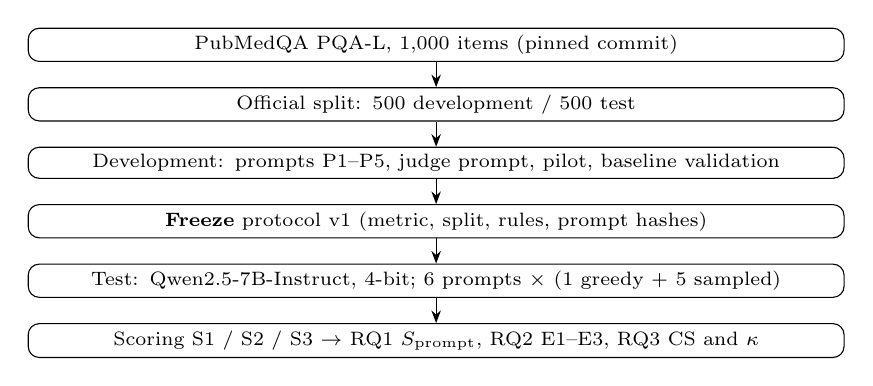
\begin{tikzpicture}[node distance=3.2mm,
  box/.style={draw, rounded corners, align=center, font=\scriptsize,
              text width=0.84\columnwidth, inner sep=2.5pt},
  arr/.style={-{Stealth[length=1.6mm]}}]
\node[box] (a) {PubMedQA PQA-L, 1{,}000 items (pinned commit)};
\node[box, below=of a] (b) {Official split: 500 development / 500 test};
\node[box, below=of b] (c) {Development: prompts P1--P5, judge prompt,
pilot, baseline validation};
\node[box, below=of c] (d) {\textbf{Freeze} protocol v1 (metric, split,
rules, prompt hashes)};
\node[box, below=of d] (e) {Test: Qwen2.5-7B-Instruct, 4-bit; 6 prompts
$\times$ (1 greedy + 5 sampled)};
\node[box, below=of e] (f) {Scoring S1 / S2 / S3 $\rightarrow$
RQ1 $\Sp$, RQ2 E1--E3, RQ3 CS and $\kappa$};
\draw[arr] (a) -- (b);
\draw[arr] (b) -- (c);
\draw[arr] (c) -- (d);
\draw[arr] (d) -- (e);
\draw[arr] (e) -- (f);
\end{tikzpicture}
\caption{Study pipeline. Everything above the freeze uses development
items only.}
\label{fig:pipeline}
\end{figure}

% =====================================================================
\section{Results}
\label{sec:results}
\subsection{Baseline validation (development items)}
Before any test run, we audited the baseline B0 on the 500 development
items. The split, the gold labels, the exact prompts (20/20 rebuilt to the
recorded token counts), the metrics (identical to scikit-learn and, with
no invalid answers, to the official evaluation script) and the records all
passed. Greedy decoding was in effect despite the model's sampling
defaults: outputs were identical under three seeds (5/5 items), while a
control with the defaults changed 5/5. A rerun in a new session reproduced
20/20 outputs. An evaluation script re-checked ID alignment, missing
values, the partition, prompt leakage and comparator settings before
computing any metric, and reproduced all reported numbers.

\begin{table}[t]
\centering
\caption{Baseline B0 on the 500 development items, with 95\% bootstrap
CIs. Gold: 276 yes / 169 no / 55 maybe.}
\label{tab:b0}
\small
\begin{tabular}{@{}lcc@{}}
\toprule
 & B0 (P0, greedy) & Always ``yes'' \\
\midrule
Accuracy & 0.588 [0.544, 0.628] & 0.552 [0.508, 0.594] \\
Macro-F1 & 0.553 [0.513, 0.590] & 0.237 [0.225, 0.248] \\
Invalid & 0 & 0 \\
Predicted yes/no/maybe & 191 / 107 / 202 & 500 / 0 / 0 \\
\bottomrule
\end{tabular}
\end{table}

Table~\ref{tab:b0} shows that B0 is above the majority control only in the
point estimate: the paired difference is $+0.036$ [$-0.022$, $+0.096$]
with 111 items right only for the control and 129 only for B0 (exact
McNemar $p = 0.27$). Its macro-F1 is far higher, because the control never
predicts ``no'' or ``maybe''. The errors are mostly hedges: of 206
errors, 170 are expert ``yes'' or ``no'' items answered ``maybe'', 23 are
expert ``maybe'' items answered yes or no, and only 13 commit to the wrong
side. When B0 commits, it is usually right (precision 0.864 for ``yes'',
0.907 for ``no'', against 0.158 for ``maybe'').

\subsection{What drives the hedging (development items)}
To locate the cause, we ran three variants on 100 development items
(55/34/11) with the same model, decoding and items, changing one factor
at a time (Table~\ref{tab:diag}, Fig.~\ref{fig:diag}). These variants are
diagnostics, not paraphrases: they change the output format, which the
paraphrases P1--P5 must not do.

\begin{table}[t]
\centering
\caption{Diagnostics on the same 100 development items. Paired comparison
with P0 (4-bit): items right only for P0 : only for the variant, exact
McNemar with Holm correction over the three tests.}
\label{tab:diag}
\small
\setlength{\tabcolsep}{3pt}
\begin{tabular}{@{}lccc@{}}
\toprule
Variant & Accuracy [95\% CI] & y/n/m & P0 : var., $p_{\mathrm{Holm}}$ \\
\midrule
P0, 4-bit & 0.56 [0.47, 0.66] & 36/23/41 & -- \\
P0, 8-bit & 0.57 [0.47, 0.67] & 37/20/43 & 4 : 5, 1.000 \\
D1, one word & 0.33 [0.24, 0.42] & 22/4/74 & 27 : 4, 0.0001 \\
D2, conclusion first & 0.72 [0.63, 0.81] & 49/28/23 & 4 : 20, 0.003 \\
Always ``yes'' & 0.55 & 100/0/0 & -- \\
\bottomrule
\end{tabular}
\end{table}

Changing the weights from 4-bit to 8-bit had no detectable effect
($+0.01$ [$-0.05$, $+0.07$]); this is not evidence of equivalence. Asking
for a one-word answer (D1) lowered accuracy by 0.23 and increased hedging
to 74 ``maybe''. Moving the conclusion field before the decision field
(D2) raised accuracy by 0.16 [0.07, 0.25] and reduced ``maybe'' from 41 to
23 (gold: 11). D2 met the rule fixed before the check ($\ge 5$ points,
$p < 0.05$, fewer ``maybe''). However, D2 was designed after seeing B0's
errors and measured on the same items, so the size of the gain is likely
overstated.

\begin{figure}[t]
\centering
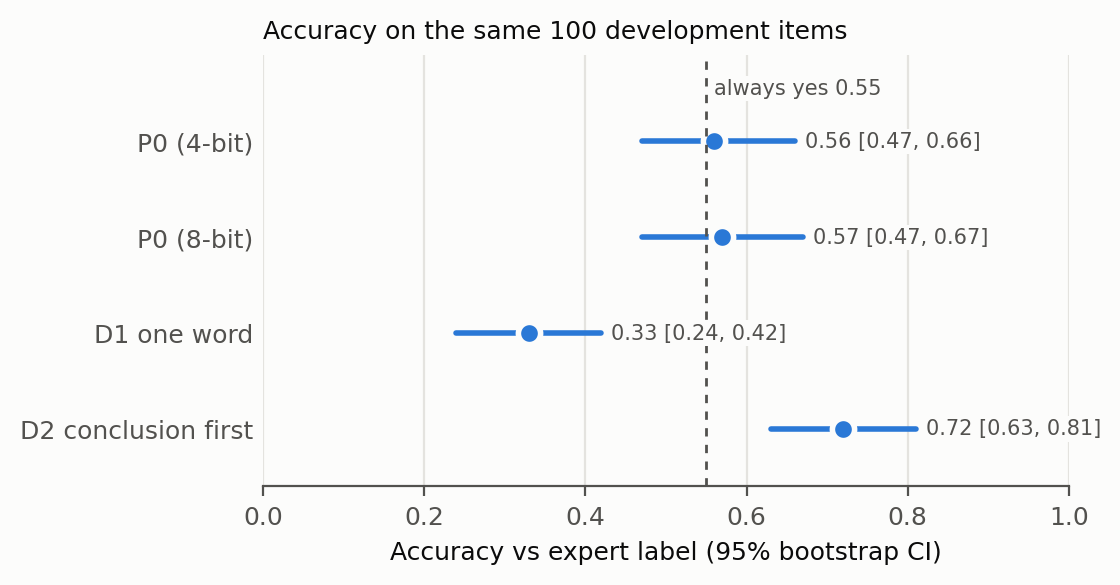
\includegraphics[width=\columnwidth]{figures/accuracy_diag100.png}\\[2pt]
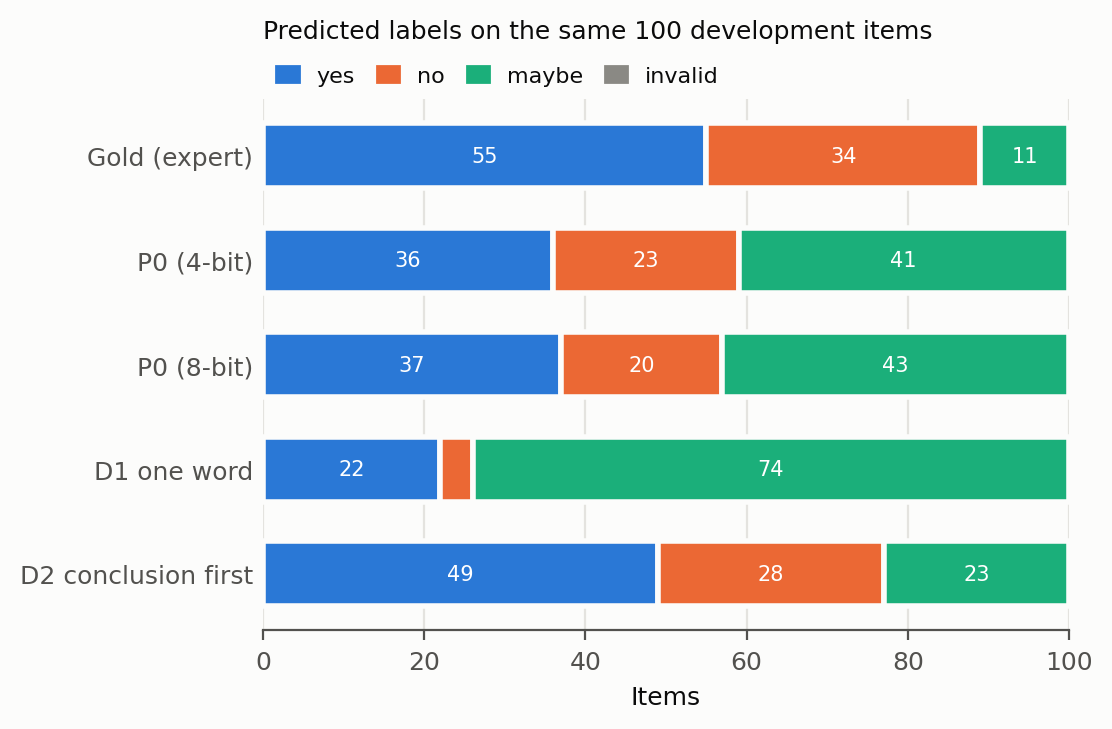
\includegraphics[width=\columnwidth]{figures/labels_diag100.png}
\caption{Diagnostics on the same 100 development items. Top: accuracy with
95\% bootstrap CI; the dashed line is the always-``yes'' control. Bottom:
predicted labels against the expert labels.}
\label{fig:diag}
\end{figure}

\subsection{RQ1: prompt versus sampling disagreement}
\subsection{RQ2: single prompt, self-consistency and multi-prompt}
\subsection{RQ3: scoring method}
\subsection{Cost}
B0 took 3.71\,s per answer (13.7 tokens/s; 31 GPU-minutes for 500
answers). The 8-bit model took 12.6\,s per answer, about 3.4 times slower,
with no detectable accuracy difference. 

% =====================================================================
\section{Discussion}
\textbf{A format effect in the baseline.} The baseline's main failure is
hedging, and it moves with the output format, not with quantisation or
parsing (there were no invalid answers, and every stored label equals a
fresh parse). \emph{Conjecture:} committing to a label before writing
anything leads the model to hedge, and writing the conclusion first acts
like a one-sentence reasoning step; D1, which allows no reasoning at all,
hedges most. This is consistent with work on reasoning before
answering~\cite{wei2022chain}, but we did not test the mechanism.
Alternative explanations remain: some abstracts without their conclusion
may truly support ``maybe'' (a single human reaches 78.0\% on the PubMedQA
test set~\cite{jin2019pubmedqa}), and the instruction ``based only on this
evidence'' may encourage caution. The D2 result does not show that D2 is a
better prompt in general. Its 0.72 is close to the 73.9\% reported by Thapa
et al.~\cite{thapa2025disentangling}, but the settings differ, so we do
not claim to reproduce it.

\textbf{Consequence for the study.} We keep P0 unchanged as the baseline,
and P1--P5 keep its field order. $\Sp$ therefore measures the effect of
\emph{instruction wording} at a baseline that hedges often. Because
samples can move between ``maybe'' and a committed label, the hedging may
inflate the within-prompt part (conjecture); we report the per-prompt
``maybe'' share with RQ1.
\textbf{Negative and null results.} B0 is not significantly more accurate
than the majority class; 8-bit and 4-bit weights are not distinguishable
at $n = 100$; and the one-word format is clearly worse. We report these as
they are.

% =====================================================================
\section{Limitations}
All results reported so far come from development items; none is a
test-set result. We study one model in 4-bit precision, one dataset and
one language, so no generalisation is claimed. Six hand-written prompts
are a sample of possible wordings. With 100 paired items, only large
differences are detectable. PubMedQA is public, so the model may have seen
the abstracts; the question-only control addresses this in the main runs
but has not been run on development items. The ``maybe'' class is small
(11 of 100 items in the diagnostics), so macro-F1 and ``maybe'' recall
are unstable. Accuracy measures agreement with the expert's label, not the
quality of the model's reasoning; the certainty field is self-reported
and was not tested for calibration. Finally, the LLM judge in RQ3 may come
from the same model family as the model under test.

% =====================================================================
\section{Conclusion}
We set out a pre-registered design to separate prompt-induced from
sampling-induced instability in LLM conclusions on biomedical evidence,
and validated its baseline on development data. The baseline is
reproducible and correctly evaluated, but it hedges on many clear items,
and this is linked to its output format rather than to quantisation.The
practical lesson so far is narrow: before measuring how stable a model's
conclusions are, check what the output format itself does to them.

\section*{Data and Code Availability}
Code, configuration, prompts and result files:

\section*{Use of AI Tools}
Claude Code (Anthropic) was used to draft code, analyses and text. Every
number was produced by code that the author ran on Colab, and every
reference was checked against its source. AI mistakes found during the
work are listed in the project's assistance log.

\bibliographystyle{IEEEtran}
\bibliography{refs}

\end{document}

